\section {Experimental Part }

\begin{figure}
\centering
\begin{tabular}{cc}
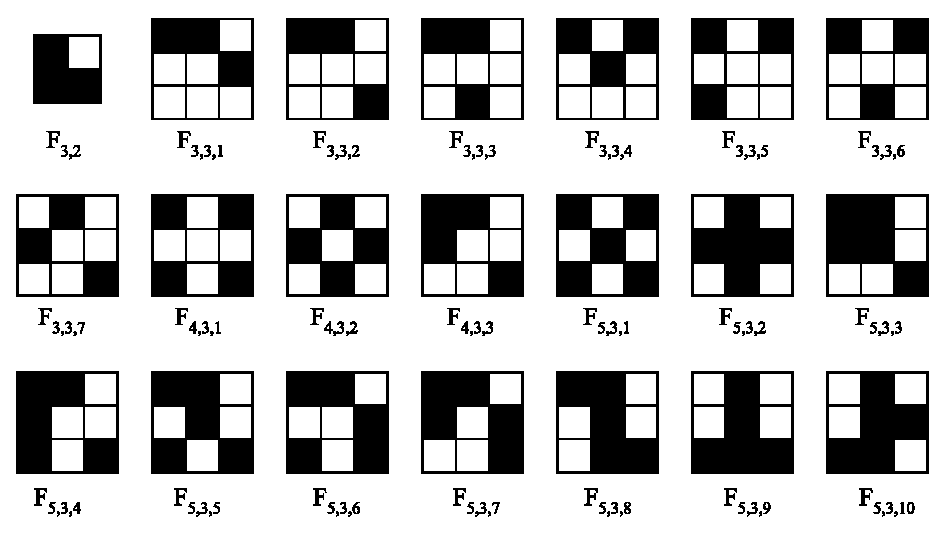
\includegraphics{involvedFractals/fractals.eps}
\end{tabular}
\caption{Table of the fractals involved in the research.}
\label{fig:involvedFractals}
\end{figure}

\begin{table}[]
\centering
\caption{Particular values of each fractal. $\alpha_{\mbox{\scriptsize{model}}}$ and $p_{\mbox{\scriptsize{value}}}$ computed for exponential model}
\vspace{2mm}
\label{tab:table1}
\begin{tabular}{|l||l|l||l|l||l|l|}
\hline
Fractal & $h$ & $D_{0}$ & $\hat{D}_{0,\mbox{\scriptsize{naive}}}$ & $\alpha_{\mbox{\scriptsize{opt}}}$ & $\alpha_{\mbox{\scriptsize{model}}}$ & $p_{\mbox{\scriptsize{value}}}$ \\ \hline \hline
$\mathrm{F_{3,2}}$ & 11 & 1,585 & 1.567 & 0,778 & 0,749 &	0,392  \\
$\mathrm{F_{3b,3}}$ & 7 & 1 & 0,982 & 1,885 & 1,886	& 0,995 \\
$\mathrm{F_{3c,3}}$ & 7 & 1 & 0,977 & 2,178 & 1,901	& 0,131 \\
$\mathrm{F_{3d,3}}$ & 7 & 1 & 0,977 & 2,004 &  1,901	& 0,667  \\
$\mathrm{F_{3e,3}}$ & 7 & 1 & 0,985 & 1,958 &  1,878	& 0,743  \\
$\mathrm{F_{3f,3}}$ & 7 & 1 & 0,976 & 1,525 &  1,904	& 0,129  \\
$\mathrm{F_{3g,3}}$ & 7 & 1 & 0,983 & 1,760 &  1,883	& 0,698  \\
$\mathrm{F_{3h,3}}$ & 7 & 1 & 0,979 & 1,873 &  1,895 &	0,929  \\
$\mathrm{F_{4a,3}}$ & 7 & 1,262 & 1,251 & 1,302 &  1,236	& 0,789  \\
$\mathrm{F_{4b,3}}$ & 7 & 1,262 & 1,248 & 1,196 &  1,242	& 0,850  \\
$\mathrm{F_{4c,3}}$ & 7 & 1,262 & 1,258 & 1,502 &  1,223	& 0,283  \\
$\mathrm{F_{5a,3}}$ & 7 & 1,465 & 1,447 & 0,871 &  0,908	& 0,653  \\
$\mathrm{F_{5b,3}}$ & 7 & 1,465 & 1,447 & 0,830 &  0,908	& 0,427  \\
$\mathrm{F_{5c,3}}$ & 7 & 1,465 & 1,451 & 0,941 &  0,903	& 0,544  \\
$\mathrm{F_{5d,3}}$ & 7 & 1,465 & 1,445 & 0,886 &  0,911	& 0,720  \\
$\mathrm{F_{5f,3}}$ & 7 & 1,465 & 1,444 & 0,864 &  0,913	& 0,367  \\
$\mathrm{F_{5g,3}}$ & 7 & 1,465 & 1,451 & 1,046 &  0,903	& 0,185  \\
$\mathrm{F_{5h,3}}$ & 7 & 1,465 & 1,453 & 1,061 &  0,900	& 0,019  \\
$\mathrm{F_{5i,3}}$ & 7 & 1,465 & 1,447 & 0,841 &  0,908	& 0,122  \\
$\mathrm{F_{5j,3}}$ & 7 & 1,465 & 1,442 & 0,755 &  0,916	& 0,009  \\
$\mathrm{F_{5k,3}}$ & 7 & 1,465 & 1,448 & 0,860 &  0,907 & 0,186  \\ \hline
\end{tabular}
\end{table}

The Revisited Box Counting technique will be tested on models of deterministic self-similar 2D fractal sets. They are generated by recursive expansion of binary matrix $\mathbb{G}_{u,v} \in \{ 0, 1 \}^{v \times v} $, where $u$ a is the number of non-zero elements (units), $v>1$ is a matrix dimension, and $v<u<v^2$. \\
\\*
Recursive expansion of $\mathbb{G}_{u,v}$ generates a binary matrix which represents fractal set $\mathbb{F}_{u,v}$ of a similarity dimension $D_{\text{S}} = D_{\text{H}} = D_{0} = D_{1} = \frac{\log{u}}{\log{v}}$. Depth $h$ of recursion depends on $v$ and should be appropriate to computer memory size. The structures involved in the research are depicted in Fig. \ref{fig:involvedFractals}\\
\\*
At first, adequate point sets of given depth $h$ were generated. Then, they were randomly rotated around the origin, and finally they were randomly shifted. Afterwards, a grid of size $a$ was put on the data points and entropy estimates were calculated. Due to physical interpretation of entropy, the estimates were averaged over 20 realizations and mean values of entropy were calculated. \\
\\*
The relationship between $\hat{D}_{\mbox{\scriptsize{naive}}}$ and optimum value of $\alpha$ was studied on the aforementioned fractals for the grid of size $a=12,16,20,...,480,500$. Results of optimization are collected in Tab. \ref{tab:table1}. We suppose, the relationship can be approximated by linear, exponential, or power model as
\begin{equation}
\label{eq:models}
\begin{split}
 \alpha &= A + B \hat{D}_{0,\mbox{\scriptsize{naive}}}, \\
 \ln \alpha &= A + B \hat{D}_{0,\mbox{\scriptsize{naive}}}, \\
 \ln \alpha &= A + B \ln \hat{D}_{0,\mbox{\scriptsize{naive}}}.
\end{split}
\end{equation}
\\*
Linearised regression was used for the estimation of unknown parameters. Results are included in Tab. \ref{tab:model_results}. The best model was the exponential and the values $\alpha_{\mbox{\scriptsize{model}}}$ and corresponding $p_{\text{value}}$ from t-test of hypothesis $\text{E}\hat{D}_{0} = D_{0}$ are also included in Tab. \ref{tab:table1}.

\begin{table}[]
\centering
\caption{Comparison of the models fitting the relationship between $\hat{D}_{0,\mbox{\scriptsize{naive}}}$ and $\alpha$}
\vspace{2mm}
\label{tab:model_results}
\begin{tabular}{r||l|l|l}
model       & A & B & r \\ \hline \hline
linear      & 3,905 & -2,066 & 0,646 \\
exponential & 2,178 & -1,571 & 0,485 \\
power       & 0,605 & -1,892 & 0,500
\end{tabular}
\end{table}